\chapter{Einleitung}

Mit dem Forschungsprojekt \gls{IKC} als Grundlage beschäftigt sich die vorliegende Arbeit vertieft mit der Analyse von Datenquellen und der Extraktion von relevanten Informationen. Aktuelle werden Datenquellen verknüpft, jedoch wird deren Inhalt noch nirgends genutzt. 

\begin{figure}[ht]
\centering
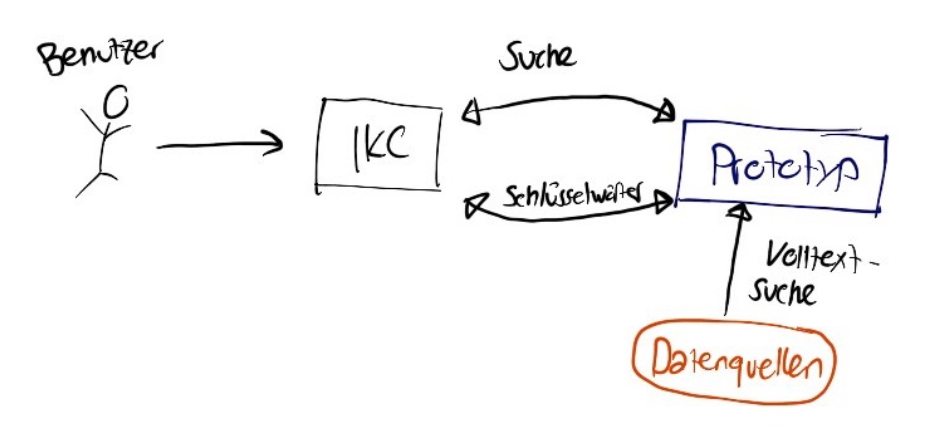
\includegraphics[width=1\textwidth]{kontextdiagramm}
\caption{Kontextdiagramm}
\label{fig:kontextdiagramm}
\end{figure}

\begin{quote}
\textit{An ounce of information is worth a pound of data.}\\
\textit{An ounce of knowledge is worth a pound of information.}\\
\textit{An ounce of understanding is worth a pound of knowledge.}\\
\end{quote}

Mit der Analyse dieser Inhalte werden zusätzliche Informationen Teil des Wissensnetzwerks. Aus Nutzung der Inhalte der bereits ver\-knüpf\-ten Datenquellen entsteht so ein Mehrwert. Dieser sorgt einerseits für eine Aufwertung des Informationsgehalts und andererseits soll er den Benutzer in der Verwendung des Prototypen unterstützen.

Die Auswertung der Datenquellen ermöglicht dem Benutzer eine plattformübergreifende Volltextsuche und präsentiert ihm automatisch eine Auswahl der relevanten Begriffe zum jeweiligen Inhalt. Dadurch wird aus einer reinen Verknüpfung von Datenquellen eine tatsächliche Integration der Informationen.

Für die Auswahl der Relevanten Begriffen werden Methoden aus der Statistik als auch aus der Sprachverarbeitung verwendert. Erstere werden verwendet um die entsprechende Relevanz eines Begriffs zu berechnen, während zweiteres für Reduktion der potentiellen Begriffe verwendet wird. Dabei werden unteranderem bekannte Sprachstrukturen, welche relevante Begriffe auszeichnen, berücksichtigt. Der Ideale relevante Begriff zeichnet sich durch eine hohe Relevanz innerhalb des Textes, aber einer niedrigen Relevanz innerhalb des ganzen \gls{Text-Korpus} aus.




Wissen und Information, cooles Zitat
% http://faculty.ung.edu/kmelton/Documents/DataWisdom.pdf

%Im Forschungsprojekt \textbf{\textit{IKC}}\footnote{\gls{Intuitive Knowledge Connectivity}} wird ein Prototyp für den Umgang mit einem plattformübergreifenden Wissensnetzwerk entwickelt. Obwohl die grundlegende Datenbasis ebenfalls in Form eines Netzwerks aufgebaut ist, wählt die Benutzeroberfläche einen anderen Ansatz: Bisher handelt es sich lediglich um eine technische Konsole. Diese macht für den Benutzer zwar alle existierenden Funktionalitäten zugänglich, jedoch ist sie weder sonderlich effizient noch benutzerfreundlich. Für einen ersten Machbarkeitsnachweis war dies ausreichend. Um den Prototypen aber einem grösseren Nutzerkreis verfügbar zu machen, gibt es Optimierungsbedarf. Auch macht es aus Sicht des Projektteams Sinn, dass die Netzwerkstruktur auch für den Benutzer sichtbar ist. Das Ziel dieser Arbeit ist darum ein Prototyping einer webbasierten Visualisierung zur intuitiven Interaktion mit einem Wissensnetzwerk.

Zum besseren Verständnis werden potentiell unbekannte oder projekt-spezifische Begriffe kursiv und fett dargestellt. Zu jedem Begriff ist eine kurze Beschreibung im Glossar (\autoref{glossar}) am Ende der Dokumentation zu finden. Im Anhang sind neben der Aufgabenstellung (\autoref{aufgabenstellung}) auch die wichtigsten Sitzungsprotokolle (\autoref{protokolle}) und das Arbeitsjounrnal (\autoref{arbeitsjournal}) beigelegt. Der dokumentierte Sourcecode\footnote{\url{https://gitlab.enterpriselab.ch/ikc/ikc-visual}} ist auf dem entsprechenden Repository der Hochschule Luzern verfügbar.


\section{Ausgangslage}

\begin{itemize}
    \item Der bestehende Prototyp \gls{ikc-core} dient als Grundlage für diese Bachelorarbeit. Mit dem Fokus der reinen Datenanalyse wird auf die Datenquellen Dropbox und Evernote verzichtet. Der resultierende Prototyp der Bachelorarbeit wird auf der bestehenden Umgebung ausgeführt.
    \item Aufgrund der bisherigen Erfahrungen wird als Programmiersprache weiterhin auf Typescript eingesetzt. Dies hat den Vorteil, dass Typescript sowohl client- als auch serverseitig lauffähig ist.
    \item Der Prototyp soll weiterhin im Browser ausgeführt werden. Jegliche Daten werden nur an benutzerdefinierten Orten gespeichert.
    \item Als Plattform wird weiterhin \gls{Dokku} eingesetzt. Diese wird für das Proof of Concept (\gls{PoC}) und für das Prototyping verwendet.
\end{itemize}

\section{Scope}\label{sec:scope} 

\begin{itemize}
    \item Da die Herkunft der Informationen für die Analyse nicht wichtig ist, beschränkt sich die Arbeit auf Text-Dateien. Versprechen die Resultate einen grossen Mehrwert können die Konzepte spä\-ter für die Verwendung mit weiteren Datenquellen erweitert werden.
    \item Um mögliche Schwierigkeiten und Hindernisse mit Dropbox auszuschliessen, wird eine neue Datenquelle und Persistenzbasis auf der Grundlage von \gls{SFTP} eingeführt.
    \item Der Projektpartner stellt die Testendaten auf Basis einer Sammlung von Wikipedia Artikeln zur Verfügung. Die Auswahl muss aufgrund der grossen Datenmenge möglicherweise eingeschränkt werden.
    \item Aufgrund der Anforderungsanalyse\footnote{{Protokoll der Anforderungsanalyse \autoref{anforderungsanalyse-mk}}} mit dem Projektpartner wurde das Projekt noch spezifischer auf die Schlüss\-el\-wort\-ex\-traktion fokussiert. Ein SFTP-Service ersetzt dabei eine Anbindungen an Dropbox und Evernote.
\end{itemize}

\section{Projektstrukturplan}
Die \autoref{fig:projektstrukturplan} gewährt einen Überblick über das Projekt. Sie stellt die wichtigsten Bereiche und Phasen dar, in welche die Arbeit grob eingegliedert werden kann:
\begin{enumerate}
    \item Die \textbf{Projektführung} beinhaltet die Planung des Vorhabens über den gegebenen Zeitraum. Ständige Kontrolle des Ist- gegenüber dem Soll-Zustand kann gegebenenfalls zur Steuerung oder Anpassungen des Zeitplans führen. Im Gegensatz zu den anderen Bereichen wird die Projektführung über die volle Projektdauer ausgeführt. Da das Projekt agil organisiert ist, liegt das Augenmerk auf der Priorisierung der Anforderungen.
    \item In der \textbf{Konzeption} werden neben den Anforderungen auch mög\-li\-che Lös\-ungs\-an\-sätz\-e in den Bereichen Architektur und Schnittstellen geprüft.
    \item Nach einer anfänglichen Recherchephase werden zum Testen bereits erste Prototypen entwickelt. So sollen mögliche Optionen überprüft und gegebenenfalls implementiert oder weiterentwickelt werden. Nach einer \textbf{Evaluation} werden die geeigneten Lösungen ausgewählt.
    \item In der \textbf{Entwicklung} werden die gesammelten Erkenntnisse gesammelt und analysiert. Wichtige Faktoren für eine erfolgreiche Umsetzung sind die Performance, die Benutzeroberfläche und die Interaktion. Grundsätzlich soll auf den zuvor entwickelten Prototypen aufgebaut werden. Zunächst wird eigenständig, also ohne Einbindung in den \gls{ikc-core} entwickelt.
    \item Sobald die Implementierung die erforderlichen Anforderungen reibungslos erfüllt, wird sie in den bestehenden \gls{ikc-core} \textbf{integriert}. Nach letzten Optimierungen sind nun alle Anforderungen werden erfüllt und es kann getestet werden.
    \item Nachdem die Entwicklungsarbeiten abgeschlossen sind, folgt der \textbf{Projektabschluss}. Dabei wird die endgültige Version des Projektreports erstellt und die Abschlusspräsentation gehalten.
\end{enumerate}

\section{Rahmenplan}
Die Rahmenplanung, basierend auf dem Projektstrukturplan (\autoref{fig:rahmenplan}), repräsentiert die zeitliche Planung des Projekts. Dabei werden Kalenderwochen anstelle von Daten oder Schulwochen verwendet. Dies aufgrund des internationalen Rahmens, der damit verbundenen Zeitverschiebung und unterschiedlichen Stundenplänen. Enthalten sind alle Projektphasen, Sprints und Meilensteine, als auch alle Lieferobjekte welche im \autoref{lieferobjekte} weiter ausgeführt werden. Die Dauer der Sprints wird bewusst unterschiedlich ausgestaltet, um den verschiedenen Projektphasen und deren Inhalten Rechnung zu tragen.
%Die Sprints dauern absichtlich unterschiedlich lange, das deshalb, weil die Länge auf\-grund der verschiedenen Projektphasen und deren Inhalt zugeordnet worden ist. Weiter werden administrative Elemente durch blaue Färbung und Entwicklungs-Elemente durch rote Färbung gekennzeichnet.

Eine grosse Rolle in der Rahmenplanung spielen die Meilensteine. Sie unterteilen das Projekt in Phasen, welche dadurch klar voneinander getrennt sind. Ebenfalls sind sie eine wichtige Orientierungshilfe im Projekt und weisen den Weg damit das Projekt erfolgreich abgeschlossen werden kann. Die \autoref{tab:meilensteine} listet die Meilensteine auf.

\section{Projektziele} \label{projektziele}
Projektziele werden definiert, um den Erfolg an einigen ausgewählten Punkten zu überprüfen und sicherstellen zu können. Sie wurden in Absprache mit dem Kunden definiert. Die Ziele sind in der folgenden \autoref{tab:projekt-ziele} aufgelistet.


%1.) Den Volltext von Dropbox-Dateien und Evernote-Notizen in IKC zu durchsuchen
%2.) Relevante Schlüsselwörter pro Dokument zu ext-rahieren
%3.) Schlüsselwörter automatisch dem Wissensnetz-werk hinzuzufügen
%4.) Dokumente mit den Schlüsselwörtern automatisch zu verknüpfen.

\begin{longtable}{|p{1cm}  | p{10.5cm}|}
  \hline
    ID &  Beschreibung \\\hline
    Z1 & Volltextsuche zusätzlich über externe Inhalte.\\\hline
    Z2 & Pro Dokument relevante Schlüsselwörter extrahieren.\\\hline
    Z3 & Extrahierte Schlüsselwörter werden automatisch dem Wissensnetzwerk hinzugefügt.\\\hline
    Z4 & Dokumente werden automatisch mit den entsprechenden Schlüsselwörtern verbunden.\\\hline
    \caption{Projektziele}
  \label{tab:projekt-ziele}
\end{longtable}

\begin{enumerate}
    \item \textbf{Z1}: Der Prototyp bietet eine Volltextsuche über den gesamten Inhalt der Dokumente einer externen Datenquelle an. Die Suchfunktion ist in den \gls{ikc-core} integriert.
    \item \textbf{Z2}: Zu den einzelnen Dokumenten extrahiert der Prototyp aus dem Text eine festgelegte Anzahl an Schlüsselwörtern.
    \item \textbf{Z3}: Diese Schlüsselwörter werden nach der Extraktion direkt teil des Wissensnetzwerkes. Diese können vom Benutzer wieder entfernt werden.
    \item \textbf{Z4}: Der Node eines Dokumentes wird automatisch mit den Node der extrahierten Schlüsselwörtern verbunden. 
\end{enumerate}

\section{Anforderungen} \label{sec:anforderungen}

Für die weitere Unterteilung in Arbeitspakete und \textit{Stories} werden die Anforderungen zunächst in Prosa gesammelt. Diese entstammen dem Kundenworkshop und der Aufgabenstellung, sind im Sinn der Projektziele (\autoref{projektziele}). Die Anforderungen werden unterschieden in funktionale und nicht-funktionale Anforderungen. Die funktionalen Anforderungen definieren direkt die Eigenschaften, (\autoref{tab:funktionale-anforderungen}). Im Gegensatz dazu definieren nicht-funktionale Anforderungen die Leistung und die Randbedingungen, aufgelistet in \autoref{tab:nicht-funktionale-anforderungen}.

Die Priorisierung erfolgt nach dem \gls{MoSCoW-System}:

\begin{longtable}{|p{1.5cm} | p{2.5cm} | p{7.2cm}|}
  \hline
    \# & Priorität & Beschreibung \\\hline
    M & Must Have & Bei dieser Anforderung handelt es sich um ein Muss, höchste Priorität.\\\hline
    S & Should Have & Diese Anforderung wird erwartet, normale Priorität.\\\hline
    C & Could Have & Tiefste Priorität, desiderata.\\\hline
    \caption{MosCow-Priorisierung}
  \label{tab:moscow}
\end{longtable}


\section{Lieferobjekte}\label{lieferobjekte}

Neben den in der Aufgabenstellung vorgegebenen Lieferobjekte (\autoref{tab:set-lieferobjekte}) sind noch zusätzliche, interne Lieferobjekte (\autoref{tab:add-lieferobjekte}) festlegt. Diese sind lediglich als Unterstützung der Projektkontrolle, eine Art Orientierungshilfe, gedacht.

